% Disappearing-tracks talk template (Beamer, 16:9, 12pt).
%
% Layout follows the group's earlier approval talk (EXO-19-010): section
% navigation bar in the footer, a source tag on each result slide, and a
% "Since <last review>" call-out. Adapted for slides built from DisappTrks_Nano
% output; see ../SKILL.md ("Conventions from the previous iteration").
%
% Every placeholder is marked TODO. Nothing here is a result: numbers, figures, and
% author/logo material must come from real outputs or the presenter. Group logos
% are NOT included -- add the approved files yourself (see \titlegraphic below).
%
% Build:  latexmk -pdf -interaction=nonstopmode -halt-on-error -outdir=build talk.tex
% Copy this file into <deck>/, point \graphicspath and \input at your figures/tables.
\documentclass[aspectratio=169,12pt]{beamer}

\usetheme{default}
\usecolortheme{default}
\usepackage{graphicx}
\usepackage{booktabs}
\usepackage{amsmath}
\usepackage{siunitx}
\usepackage{tikz}
\usetikzlibrary{arrows.meta,positioning,calc}
\graphicspath{{../figures/}}

% ------------------------------------------------------------------ colors
\definecolor{navbar}{RGB}{23,73,127}      % footer bar
\definecolor{sourcegreen}{RGB}{40,160,40} % source tag
\definecolor{sincered}{RGB}{200,30,30}    % "since last review" box
\setbeamercolor{frametitle}{fg=black,bg=white}
\setbeamerfont{frametitle}{size=\large,series=\bfseries}
\setbeamercolor{section in head/foot}{fg=white,bg=navbar}
\setbeamercolor{title in head/foot}{fg=white,bg=black}
\setbeamercolor{structure}{fg=navbar}
\setbeamertemplate{navigation symbols}{}
\setbeamertemplate{itemize items}[circle]

% ------------------------------------------------------- footer: section nav
% Section names come from \section{...}; the current one is highlighted.
\setbeamertemplate{footline}{%
  \leavevmode\hbox{%
    \begin{beamercolorbox}[wd=.55\paperwidth,ht=3ex,dp=1.2ex,left]{section in head/foot}%
      \hspace*{1em}\insertsectionnavigationhorizontal{.53\paperwidth}{}{}%
    \end{beamercolorbox}%
    \begin{beamercolorbox}[wd=.45\paperwidth,ht=3ex,dp=1.2ex,right]{title in head/foot}%
      \scriptsize
      \insertshorttitle\ \ {\footnotesize\insertframenumber}\hspace*{1em}%
    \end{beamercolorbox}}%
}

% ------------------------------------------------------------------- macros
% One-line takeaway under a figure or table.
\newcommand{\takeaway}[1]{\par\vspace{10pt}\centering\small\textbf{#1}\par}

% "Since <last review stage>" call-out, bottom-right above the footer.
\newcommand{\sincebox}[1]{%
  \begin{tikzpicture}[remember picture,overlay]
    \node[anchor=south east,draw=sincered,text=sincered,align=center,inner sep=4pt,
          font=\small] at ($(current page.south east)+(-0.3cm,1.1cm)$) {#1};
  \end{tikzpicture}}

% Figure that degrades to a labelled placeholder box if the file is missing, so the
% template compiles before any real figures exist. Size by HEIGHT (see hep-slides).
\newcommand{\slidefig}[2][0.66\textheight]{%
  \IfFileExists{#2}{\includegraphics[height=#1]{#2}}%
  {\fbox{\parbox[c][#1][c]{0.45\textwidth}{\centering TODO figure:\\ \texttt{\detokenize{#2}}}}}}

% Table that degrades to a placeholder if the .tex file is missing.
\newcommand{\slidetable}[1]{%
  \IfFileExists{#1}{\input{#1}}%
  {\fbox{TODO table: \texttt{\detokenize{#1}}}}}

% Physics shorthand
\newcommand{\ptmiss}{\ensuremath{p_T^{\mathrm{miss,\,no\,\mu}}}}
\newcommand{\nlayers}{\ensuremath{n_{\mathrm{layers}}}}

\title[Disappearing tracks]{Disappearing-Track Search: Analysis Overview}
\subtitle{Signal, selection, and background methods}
\author[M. Joyce]{Matt Joyce}
\institute[OSU]{The Ohio State University}
\date{Group meeting}

\begin{document}

\begin{frame}\titlepage\end{frame}

% ------------------------------------------------------------------ Signal
\section{Intro}
\begin{frame}{A long-lived chargino looks like a track that stops}
  \begin{itemize}
    \item Wino/higgsino-like charginos, nearly degenerate with the lightest neutralino
    \item Chargino travels $\sim$cm through the tracker, then decays to an
          undetectably soft pion and an invisible neutralino
    \item Signature: an isolated, high-$p_T$ track with \textbf{no hits in the outer layers}
    \item Produced recoiling against initial-state radiation, so the event has
          large \ptmiss{}
  \end{itemize}
  \takeaway{The search is a counting experiment in the disappearing-track signal region}
\end{frame}

\begin{frame}{The search requires large missing energy and a vanishing track}
  \begin{itemize}
    \item HLT MET trigger, then offline \ptmiss{} $> 120$ GeV with
          $|\Delta\phi(\text{leading jet},\, \ptmiss{})| > 0.5$
    \item Candidate track: tight quality, isolated, and fiducial (next slide)
    \item Disappearance: $\ge 3$ missing outer hits, calorimeter energy $< 10$ GeV
    \item Results binned by the track's number of layers with hits:
          \texttt{NLayers4}, \texttt{NLayers5}, \texttt{NLayers6plus}
  \end{itemize}
  \takeaway{Fewer measured layers means a shorter-lived candidate, and a different background mix}
\end{frame}

% ------------------------------------------------------------ Selection
\section{Selection}
\begin{frame}{The candidate-track selection is a short list of tight cuts}
  \centering
  \renewcommand{\arraystretch}{0.85}
  \begin{tabular}{p{0.34\textwidth}p{0.5\textwidth}}
    \toprule
    Requirement & Cut \\
    \midrule
    Kinematics & $p_T > 55$ GeV, $|\eta| < 2.1$ \\
    Fiducial & Outside ECAL crack, DT/CSC/TOB gaps; electron/muon fiducial maps \\
    Hits & $\ge 4$ pixel, $\ge 4$ valid; no missing inner/middle hits \\
    Isolation & Charged relative isolation $< 0.05$ \\
    Impact parameter & $|d_0| < 0.02$ cm, $|d_z| < 0.5$ cm \\
    Jet / lepton veto & $\Delta R(\text{track, jet}) > 0.5$; $\Delta R > 0.15$ from $e$, $\mu$, $\tau_h$ \\
    Disappearance & $\ge 3$ missing outer hits; calo energy $< 10$ GeV \\
    \bottomrule
  \end{tabular}
  \takeaway{From \texttt{search\_track\_mask} in \texttt{DisappTrks\_Nano}}
\end{frame}

\begin{frame}{\texttt{highPurity} and a dE/dx cut are now part of the selection}
  \begin{itemize}
    \item Required since 2026-09-17: the track \texttt{highPurity} bit
    \item Plus a max/median dE/dx cut, for \texttt{NLayers4} and \texttt{NLayers5} only
    \item Motivation: reject fake tracks, weighed against the signal efficiency it costs
          per layer bin
    \item \texttt{NLayers6plus} tracks always pass the dE/dx term
  \end{itemize}
  \takeaway{Background numbers later in this talk are the 2026-09-17 \texttt{\_dedx} outputs}
\end{frame}

% ---------------------------------------------------------- Backgrounds
\section{Backgrounds}
\begin{frame}{Three backgrounds, all estimated from data}
  \centering
  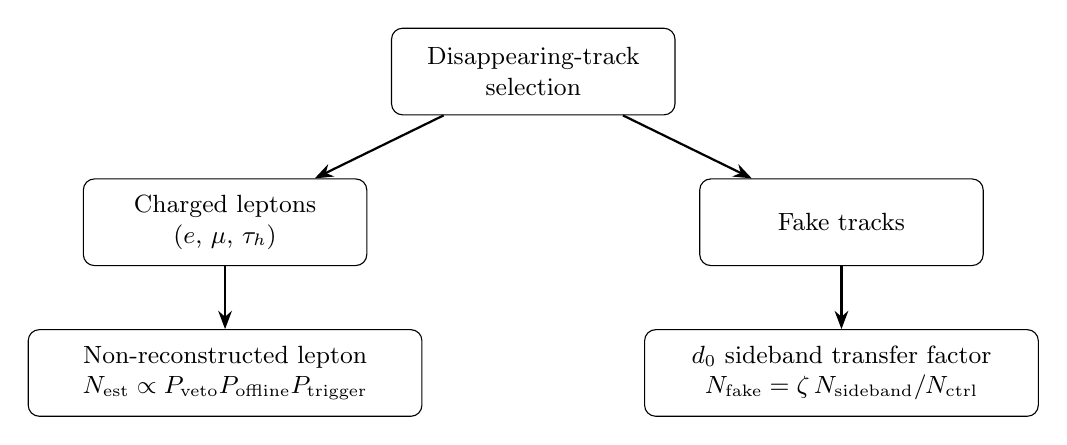
\begin{tikzpicture}[
      box/.style={rectangle, draw, rounded corners, align=center, minimum height=1.1cm,
                  minimum width=3.6cm, font=\small},
      arr/.style={-{Stealth}, thick}]
    \node[box] (sel) {Disappearing-track\\selection};
    \node[box, below left=0.8cm and 0.3cm of sel] (lep) {Charged leptons\\($e$, $\mu$, $\tau_h$)};
    \node[box, below right=0.8cm and 0.3cm of sel] (fake) {Fake tracks};
    \node[box, below=0.8cm of lep, minimum width=5cm] (lm) {Non-reconstructed lepton\\$N_{\mathrm{est}} \propto P_{\mathrm{veto}} P_{\mathrm{offline}} P_{\mathrm{trigger}}$};
    \node[box, below=0.8cm of fake, minimum width=5cm] (fm) {$d_0$ sideband transfer factor\\$N_{\mathrm{fake}} = \zeta \, N_{\mathrm{sideband}} / N_{\mathrm{ctrl}}$};
    \draw[arr] (sel) -- (lep); \draw[arr] (sel) -- (fake);
    \draw[arr] (lep) -- (lm);  \draw[arr] (fake) -- (fm);
  \end{tikzpicture}
  \takeaway{Each is measured in a control region, then applied to the search sample}
\end{frame}

\begin{frame}{A lepton that fails reconstruction looks like a disappearing track}
  \begin{itemize}
    \item The lepton leaves a track but is not reconstructed as a lepton
    \item It must also pass the offline and HLT \ptmiss{} requirements
    \item Estimate per flavor (dissertation Eq.~7.9):
  \end{itemize}
  \[
    N_{\mathrm{est}}^{\ell}
      = \frac{N_{\mathrm{ctrl}}^{\ell}}{\varepsilon_{\mathrm{trig}}^{\ell}}
        \, P_{\mathrm{veto}} \, P_{\mathrm{offline}} \, P_{\mathrm{trigger}}
  \]
  \takeaway{Three measured probabilities, times a control-sample count}
\end{frame}

\begin{frame}{Each probability is measured in its own control sample}
  \small
  \begin{tabular}{p{0.15\textwidth}p{0.36\textwidth}p{0.36\textwidth}}
    \toprule
    Term & Question answered & How measured \\
    \midrule
    $P_{\mathrm{veto}}$ & Track passes the lepton non-reconstruction veto & Tag-and-probe; same-sign subtraction removes Drell--Yan/fake contamination \\
    $P_{\mathrm{offline}}$ & Passes offline \ptmiss{} and $\Delta\phi$ cuts & Single-lepton samples; lepton re-treated as invisible \\
    $P_{\mathrm{trigger}}$ & Passes HLT MET given offline & Trigger-efficiency curve convolved with the \ptmiss{} spectrum \\
    \bottomrule
  \end{tabular}
  \normalsize
  \takeaway{Taus need extra steps: next two slides}
\end{frame}

\begin{frame}{Taus need two decay channels to measure $P_{\mathrm{veto}}$}
  \begin{itemize}
    \item Tag-and-probe with $\tau\to e\nu\nu$ (EGamma dataset) and
          $\tau\to\mu\nu\nu$ (Muon dataset)
    \item $M_T(\ptmiss{},\,\text{lepton}) < 40$ GeV suppresses $W$+jets
    \item The $\Delta R(\text{track, jet}) > 0.5$ requirement is dropped: a
          hadronic tau decay is expected near a jet
    \item Same-sign subtraction, as for electrons and muons
    \item Raw counts from the two legs are combined first, then the ratio
          is formed; two finished per-leg estimates are not averaged
  \end{itemize}
\end{frame}

\begin{frame}{The tau normalization comes from a muon+tau cross-trigger}
  \begin{itemize}
    \item Run 3 has no low-$p_T$ single-tau trigger
    \item Instead: $P(\tau) = N_{\mu+\tau} / N_{\mu}$, the ratio of a muon+tau
          cross-trigger to a muon-only trigger (dissertation Eqs.~7.7--7.8)
    \item For 4 and 5 layers, statistics are too low: these two probabilities are
          taken from the combined-layer sample
  \end{itemize}
  \centering\small\renewcommand{\arraystretch}{0.9}
  \begin{tabular}{p{0.42\textwidth}p{0.42\textwidth}}
    \toprule
    Job & Provides \\
    \midrule
    \texttt{tau\_mu\_pveto}, \texttt{tau\_ele\_pveto} & $P_{\mathrm{veto}}$ pair counts, both legs \\
    \texttt{tau\_pmiss\_poffline} & $N_{\mathrm{ctrl}}$, $P_{\mathrm{offline}}$, $P_{\mathrm{trigger}}$ \\
    \texttt{tau\_trigger\_probability} & $P(\tau)$ \\
    \bottomrule
  \end{tabular}
\end{frame}

\begin{frame}{Fake tracks are estimated from the $d_0$ sideband}
  \begin{itemize}
    \item Fakes have a broad $|d_0|$ distribution; real tracks are peaked at zero
    \item Control region: $Z\to\mu\mu$ or $Z\to ee$ events
    \item Transfer factor $\zeta$: fit to the folded $|d_0|$ distribution relates the
          signal window ($<0.02$ cm) to the sideband ($0.05$--$0.50$ cm)
  \end{itemize}
  \[
    P_{\mathrm{fake}} = \zeta \, \frac{N_{\mathrm{sideband}}}{N_{\mathrm{ctrl}}},
    \qquad N_{\mathrm{fake}} = P_{\mathrm{fake}} \, N_{\mathrm{basic}}
  \]
  \takeaway{Measured per layer bin, per control region}
\end{frame}

\begin{frame}{The methods were validated in simulation}
  \begin{itemize}
    \item Lepton closure (dissertation): $t\bar t$ and $Z\to\ell\ell$ MC with relaxed
          selections; estimate agrees with the observed non-reconstructed-lepton
          count within $1\sigma$ in all layer bins and flavors
    \item Nano-tier migration cross-checks against the legacy CMSSW code
  \end{itemize}
  \takeaway{Closure was shown before \texttt{highPurity}; repeating it under the current selection is open}
\end{frame}

% --------------------------------------------------------------- Results
\section{Results}
\begin{frame}{Fake tracks dominate at 4 layers, leptons at 6 or more}
  \centering\footnotesize\renewcommand{\arraystretch}{0.8}
  \begin{tabular}{llccc}
\toprule
 & & \multicolumn{3}{c}{Expected Backgrounds} \\
Run Period & $n_{\mathrm{layers}}$ & Leptons & Spurious Tracks & Total \\
\midrule
2022CD & 4 & $0^{+0.066}_{-0}$ & 2.6 $\pm$ 1.1 & 2.6 $\pm$ 1.1 \\
 & 5 & 0.130 $\pm$ 0.067 & 0.16 $\pm$ 0.13 & 0.29 $\pm$ 0.15 \\
 & $\geq 6$ & 1.23 $\pm$ 0.25 & 0.082 $\pm$ 0.088 & 1.31 $\pm$ 0.26 \\
\midrule
2022EFG & 4 & 0.45 $\pm$ 0.34 & 7.3 $\pm$ 1.3 & 7.8 $\pm$ 1.3 \\
 & 5 & 0.18 $\pm$ 0.11 & 0.79 $\pm$ 0.27 & 0.97 $\pm$ 0.30 \\
 & $\geq 6$ & 3.32 $\pm$ 0.44 & $0^{+0.089}_{-0}$ & 3.32 $\pm$ 0.45 \\
\midrule
2023C & 4 & 0.21 $\pm$ 0.24 & 3.21 $\pm$ 0.71 & 3.42 $\pm$ 0.75 \\
 & 5 & 0.39 $\pm$ 0.15 & 0.56 $\pm$ 0.19 & 0.95 $\pm$ 0.24 \\
 & $\geq 6$ & 3.48 $\pm$ 0.45 & $0^{+0.053}_{-0}$ & 3.48 $\pm$ 0.46 \\
\midrule
2023D & 4 & 0.000 $\pm$ 0.037 & 1.55 $\pm$ 0.43 & 1.55 $\pm$ 0.43 \\
 & 5 & 0.172 $\pm$ 0.079 & 0.193 $\pm$ 0.097 & 0.36 $\pm$ 0.12 \\
 & $\geq 6$ & 0.38 $\pm$ 0.16 & $0^{+0.044}_{-0}$ & 0.38 $\pm$ 0.16 \\
\bottomrule
\end{tabular}

  \vspace{-4pt}\takeaway{2022--2023, statistical uncertainties only}
\end{frame}

\begin{frame}{The 2024--2026 periods follow the same pattern}
  \centering\footnotesize\renewcommand{\arraystretch}{0.8}
  \begin{tabular}{llccc}
\toprule
 & & \multicolumn{3}{c}{Expected Backgrounds} \\
Run Period & $n_{\mathrm{layers}}$ & Leptons & Spurious Tracks & Total \\
\midrule
2024 & 4 & 0.26 $\pm$ 0.35 & 23.2 $\pm$ 2.0 & 23.5 $\pm$ 2.0 \\
 & 5 & 0.27 $\pm$ 0.16 & 2.61 $\pm$ 0.40 & 2.88 $\pm$ 0.43 \\
 & $\geq 6$ & 3.15 $\pm$ 0.41 & 0.24 $\pm$ 0.11 & 3.39 $\pm$ 0.43 \\
\midrule
2025 & 4 & 0.20 $\pm$ 0.31 & 28.9 $\pm$ 1.9 & 29.1 $\pm$ 1.9 \\
 & 5 & 0.32 $\pm$ 0.20 & 3.39 $\pm$ 0.40 & 3.71 $\pm$ 0.44 \\
 & $\geq 6$ & 7.77 $\pm$ 0.58 & 0.182 $\pm$ 0.082 & 7.95 $\pm$ 0.59 \\
\midrule
2026 & 4 & 0.11 $\pm$ 0.12 & 7.19 $\pm$ 0.94 & 7.30 $\pm$ 0.95 \\
 & 5 & 0.019 $\pm$ 0.035 & 0.70 $\pm$ 0.17 & 0.72 $\pm$ 0.18 \\
 & $\geq 6$ & 0.78 $\pm$ 0.19 & 0.070 $\pm$ 0.050 & 0.85 $\pm$ 0.19 \\
\bottomrule
\end{tabular}

  \takeaway{2025 is largest: $29.1 \pm 1.9$ (4 layers), $7.95 \pm 0.59$ ($\geq 6$); statistical only}
\end{frame}

% ---------------------------------------------------------------- Status
\section{Conclusion}
\begin{frame}{Backgrounds are estimated; systematics, closure and limits remain}
  \centering\small
  \begin{tabular}{p{0.28\textwidth}p{0.5\textwidth}}
    \toprule
    Item & State \\
    \midrule
    Signal selection & \texttt{highPurity} + dE/dx in production selection \\
    Fake-track background & Estimates produced for 2022--2026 (2026-09-17 \texttt{\_dedx} outputs) \\
    Lepton backgrounds & Estimates produced for 2022--2026 (same outputs) \\
    Search-region yields & \texttt{search\_region} mode verified end to end \\
    Limits & No datacard built yet \\
    \bottomrule
  \end{tabular}
\end{frame}

\begin{frame}{Three steps to a first result}
  \begin{itemize}
    \item Add systematic uncertainties (tables are statistical only)
    \item Repeat the closure tests under the current selection
    \item Build the first datacard from \texttt{search\_region}
  \end{itemize}
\end{frame}

% ---------------------------------------------------------------- Backup
\appendix
\section*{Backup}
\begin{frame}[noframenumbering]{Backup: fake-track estimates, 2022--2023}
  \centering\scriptsize
  \begin{tabular}{llrrrr}
\toprule
run period & $n_{\mathrm{layers}}$ & $P_{\mathrm{fake}}(Z\to\mu\mu)$ & $P_{\mathrm{fake}}(Z\to ee)$ & $N^{\mathrm{fake}}_{\mathrm{est}}(Z\to\mu\mu)$ & $N^{\mathrm{fake}}_{\mathrm{est}}(Z\to ee)$ \\
\midrule
2022CD & 4 & $(2.18 \pm 0.93) \times 10^{-6}$ & $(8.1 \pm 3.7) \times 10^{-7}$ & $2.6 \pm 1.1$ & $0.97 \pm 0.45$ \\
 & 5 & $(1.4 \pm 1.1) \times 10^{-7}$ & $(1.01 \pm 0.81) \times 10^{-7}$ & $0.16 \pm 0.13$ & $0.121 \pm 0.098$ \\
 & $\geq 6$ & $(6.8 \pm 7.3) \times 10^{-8}$ & $(5.0 \pm 5.4) \times 10^{-8}$ & $0.082 \pm 0.088$ & $0.060 \pm 0.065$ \\
\midrule
2022EFG & 4 & $(1.53 \pm 0.27) \times 10^{-6}$ & $(10.0 \pm 2.3) \times 10^{-7}$ & $7.3 \pm 1.3$ & $4.8 \pm 1.1$ \\
 & 5 & $(1.65 \pm 0.57) \times 10^{-7}$ & $(1.27 \pm 0.53) \times 10^{-7}$ & $0.79 \pm 0.27$ & $0.60 \pm 0.25$ \\
 & $\geq 6$ & $(0.0 \pm 1.9) \times 10^{-8}$ & $(0.0 \pm 2.1) \times 10^{-8}$ & $0.000 \pm 0.089$ & $0.000 \pm 0.098$ \\
\midrule
2023C & 4 & $(1.11 \pm 0.25) \times 10^{-6}$ & $(6.0 \pm 2.1) \times 10^{-7}$ & $3.21 \pm 0.71$ & $1.74 \pm 0.61$ \\
 & 5 & $(1.92 \pm 0.66) \times 10^{-7}$ & $(1.29 \pm 0.59) \times 10^{-7}$ & $0.56 \pm 0.19$ & $0.37 \pm 0.17$ \\
 & $\geq 6$ & $(0.0 \pm 1.8) \times 10^{-8}$ & $(1.4 \pm 1.5) \times 10^{-8}$ & $0.000 \pm 0.053$ & $0.041 \pm 0.044$ \\
\midrule
2023D & 4 & $(1.02 \pm 0.28) \times 10^{-6}$ & $(8.7 \pm 3.5) \times 10^{-7}$ & $1.55 \pm 0.43$ & $1.32 \pm 0.53$ \\
 & 5 & $(1.27 \pm 0.64) \times 10^{-7}$ & $(1.30 \pm 0.86) \times 10^{-7}$ & $0.193 \pm 0.097$ & $0.20 \pm 0.13$ \\
 & $\geq 6$ & $(0.0 \pm 2.9) \times 10^{-8}$ & $(0.0 \pm 4.9) \times 10^{-8}$ & $0.000 \pm 0.044$ & $0.000 \pm 0.075$ \\
\bottomrule
\end{tabular}

  \takeaway{Both control regions shown; the total uses $Z\to\mu\mu$}
\end{frame}

\begin{frame}[noframenumbering]{Backup: fake-track estimates, 2024--2026}
  \centering\scriptsize
  \begin{tabular}{llrrrr}
\toprule
run period & $n_{\mathrm{layers}}$ & $P_{\mathrm{fake}}(Z\to\mu\mu)$ & $P_{\mathrm{fake}}(Z\to ee)$ & $N^{\mathrm{fake}}_{\mathrm{est}}(Z\to\mu\mu)$ & $N^{\mathrm{fake}}_{\mathrm{est}}(Z\to ee)$ \\
\midrule
2024 & 4 & $(1.20 \pm 0.10) \times 10^{-6}$ & $(1.30 \pm 0.14) \times 10^{-6}$ & $23.2 \pm 2.0$ & $25.2 \pm 2.7$ \\
 & 5 & $(1.35 \pm 0.21) \times 10^{-7}$ & $(9.3 \pm 2.2) \times 10^{-8}$ & $2.61 \pm 0.40$ & $1.80 \pm 0.42$ \\
 & $\geq 6$ & $(1.22 \pm 0.55) \times 10^{-8}$ & $(4.4 \pm 4.4) \times 10^{-9}$ & $0.24 \pm 0.11$ & $0.086 \pm 0.086$ \\
\midrule
2025 & 4 & $(1.64 \pm 0.11) \times 10^{-6}$ & $(1.58 \pm 0.14) \times 10^{-6}$ & $28.9 \pm 1.9$ & $27.9 \pm 2.5$ \\
 & 5 & $(1.92 \pm 0.22) \times 10^{-7}$ & $(1.27 \pm 0.23) \times 10^{-7}$ & $3.39 \pm 0.40$ & $2.24 \pm 0.40$ \\
 & $\geq 6$ & $(1.03 \pm 0.47) \times 10^{-8}$ & $(2.01 \pm 0.83) \times 10^{-8}$ & $0.182 \pm 0.082$ & $0.35 \pm 0.15$ \\
\midrule
2026 & 4 & $(1.85 \pm 0.24) \times 10^{-6}$ & $(2.14 \pm 0.44) \times 10^{-6}$ & $7.19 \pm 0.94$ & $8.3 \pm 1.7$ \\
 & 5 & $(1.80 \pm 0.45) \times 10^{-7}$ & $(2.11 \pm 0.92) \times 10^{-7}$ & $0.70 \pm 0.17$ & $0.82 \pm 0.36$ \\
 & $\geq 6$ & $(1.8 \pm 1.3) \times 10^{-8}$ & $(3.5 \pm 3.6) \times 10^{-8}$ & $0.070 \pm 0.050$ & $0.14 \pm 0.14$ \\
\bottomrule
\end{tabular}

\end{frame}

\begin{frame}[noframenumbering]{Backup: $d_0$ fit, 2025 $Z\to\mu\mu$, 4 layers}
  \centering
  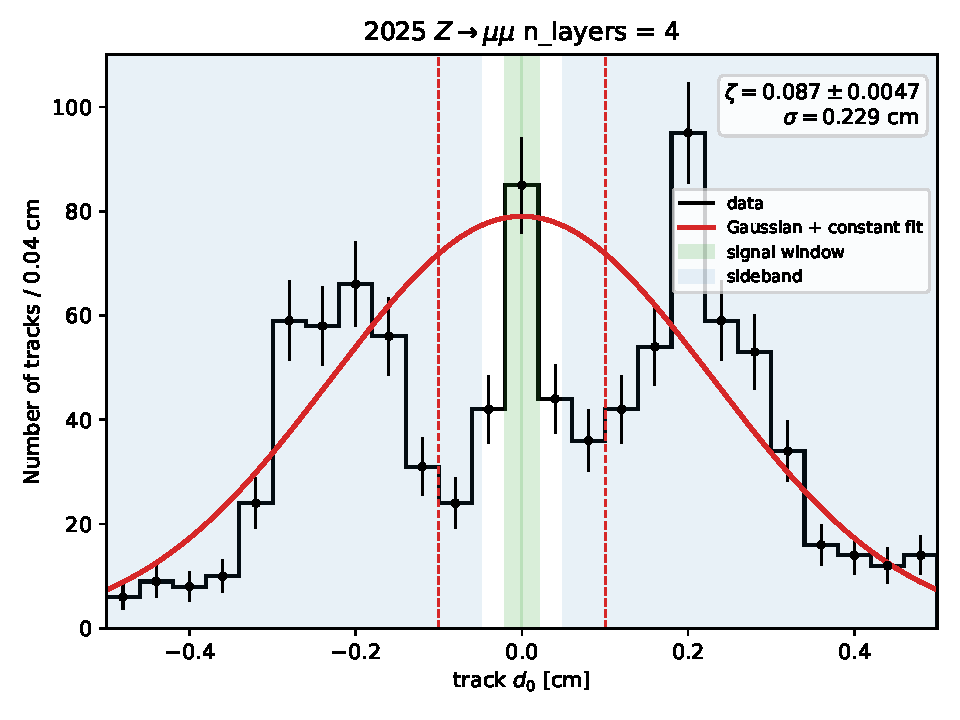
\includegraphics[height=0.72\textheight]{fake_zmumu_fit_2025.pdf}
\end{frame}

\begin{frame}[noframenumbering]{Backup: implementation}
  \begin{itemize}
    \item \texttt{DisappTrks\_Nano}: PocketCoffea-based, one \texttt{DISAPPTRKS\_CATEGORY\_MODE}
          per background and study
    \item Lepton: \texttt{*\_pveto}, \texttt{*\_pmiss\_poffline}, \texttt{fiducial\_maps}
    \item Fake tracks: \texttt{fake\_tracks} (\texttt{basic}, \texttt{zmumu}, \texttt{zee})
    \item Signal: \texttt{signal\_acceptance}, \texttt{search\_region}
  \end{itemize}
\end{frame}

\end{document}
